\documentclass[10pt]{beamer}
\usepackage{packages}
\setbeamertemplate{caption}[numbered]

\linespread{1.15}
\setlength\parindent{0pt}
\let\oldcaption\caption
\def\caption#1{\oldcaption{\centering#1}}

\setbeamertemplate{navigation symbols}{}
\usefonttheme{default}
\usefonttheme[onlymath]{serif}
\usepackage{DejaVuSansCondensed}

\usetheme{Madrid}


\title[Эффект хребта (ridge effect)]{
	Эффект хребта (ridge effect) в многочастичных корреляциях в $pp$ соударениях с большой множественностью и его возможные объяснения
}
\author[Керим Гусейнов]{Керим Гусейнов \\ Email: guseynovkerim@gmail.com}
\institute[]{Московский государственный университет, физический факультет}
\date{19 ноября 2019}

\def\hfillstar{\hspace*{0pt}\hfill\hspace*{0pt}}
\def\MyCite#1{\hspace*{-7pt}\rotatebox{90}{\footnotesize [#1]}}
\def\MyCiteHor#1{\footnotesize [#1] \normalsize}
\def\d{\mathrm{d}}
\let\phi\varphi


\begin{document}
\frame{
	\titlepage
}

\frame{
	\frametitle{Псевдобыстрота и азимутальный угол}
	\begin{columns}
	\column{.5\linewidth}{
	Псевдобыстрота $\eta$ -- кинематически удобная характеристика движения релятивистской частицы. Для ультрарелятивистских частиц она еще удобнее. 
	}
	\column{.5\linewidth}{
	Обычная быстрота $\psi$ определяется как $\tanh\psi = v/c$. Псевдобыстрота -- как $\tanh\eta = v_L/v \;\Rightarrow \eta = -\frac{1}{2}\ln\frac{v-v_L}{v+v_L} $ $$\eta = -\frac{1}{2}\ln\frac{1-\cos\theta}{1+\cos\theta} = -\ln\tg\frac{\theta}{2}$$
	}
	\end{columns}
	\centering
	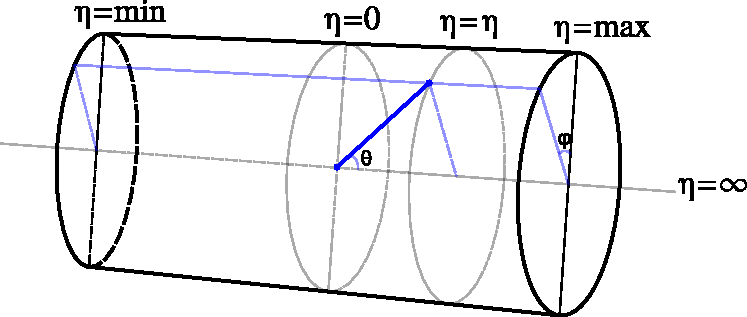
\includegraphics[height=.5\textheight]{figs/detector-eta-phi}
}

\frame{
	\frametitle{Что показывают на графиках}
	Число частиц, регистрируемых детектором в какой-то области, зависит не только от геометрии распределения частиц, но и от эффективности детектора в этой области. Чтобы как-то исправить ситуацию, не уничтожая физические корреляции между частицами, принято рассматривать отношение 
	$$C(\Delta\eta, \Delta\phi) = \frac{S(\Delta\eta, \Delta\phi)}{B(\Delta\eta, \Delta\phi)},$$
	где $S$ -- число пар частиц с $\Delta\eta$, $\Delta\phi$, выбранных в одном событии, а $B$ -- выбранных в разных, но похожих событиях. 

	%$C$, таким образом, отражает многочасичные корреляции -- избыток или недостаток пар, разнесенных в пространстве на $\Delta\eta$, $\Delta\phi$. 

	Если, например, в соударениях с большой вероятностью рождается 3 струи, то, очевидно, абсолютные значения их углов в пространстве никак не связаны в двух разных событиях. Тогда усреднение по смешанным событиям уничтожит информацию о трех струях в $B$, но не уничтожит в $S$.
}

\frame{
	\frametitle{Картина при малой множественности}
	\begin{columns}
	\column{.45\linewidth}{
	\hfillstar \MyCiteHor{arXiv:1009.4122}\\
	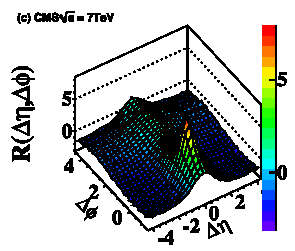
\includegraphics[width=\linewidth]{figs/low-mul}
	Многочастичные корреляции при малой множественности -- распады частиц и закон сохранения импульса. 
	}
	\column{.55\linewidth}{
	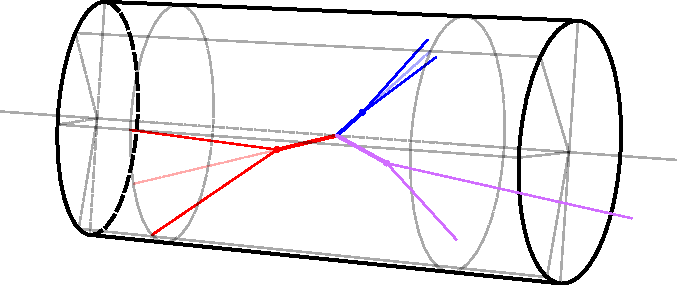
\includegraphics[width=\linewidth]{figs/decays.pdf}
	\vskip\baselineskip
	При распаде одна частица становится одной или более парами, которые имеют очевидный пик при $\Delta\phi=0$, $\Delta\eta=0$, а также в целом сосредоточены вблизи $\Delta\eta=0$, поскольку пары с большим $\Delta\eta$ регистрируются менее охотно. 
	}
	\end{columns}
}

\frame{
	\frametitle{Появление хребта в $pp$ соударениях}
	\centering
	\MyCite{arXiv:1009.4122}
	\hfillstar
	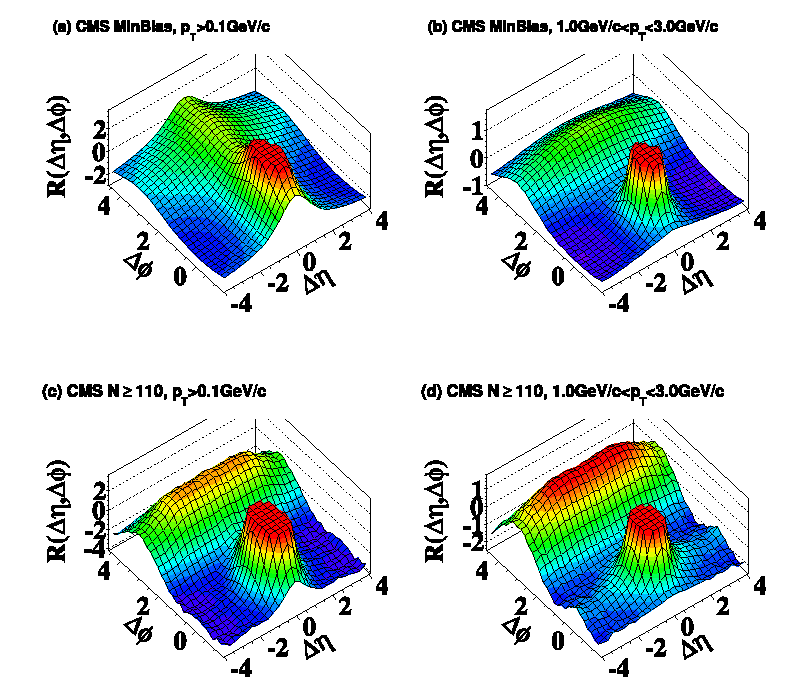
\includegraphics[width=.76\linewidth]{figs/CMS-10.pdf}
	\hfillstar
}

\frame{
	\frametitle{Пик около (0,0) и хребет при $\phi=\pi$}
	\vskip\baselineskip
	\hfillstar
	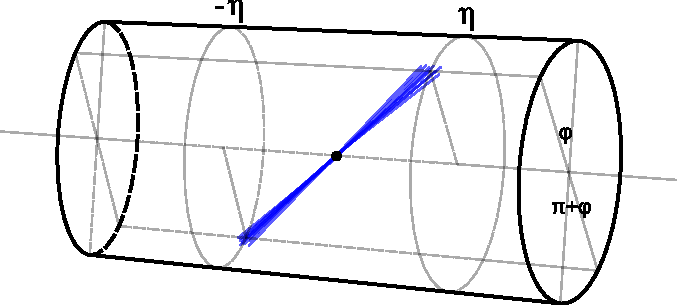
\includegraphics[width=.9\linewidth]{figs/jets}
	\hfillstar
	\vskip\baselineskip
	Для пар частиц в одной струе $\Delta\phi\approx0$, $\Delta\eta\approx0$, а в противоположных -- $\Delta\phi\approx\pi$, $\Delta\eta\approx2\eta$.
	\vskip10pt
}

\frame{
	\frametitle{Хребты в столкновениях тяжелых ионов}
	\begin{columns}
	\column{.45\linewidth}{\hspace*{-2pt}
		Здесь явление односторонних дальних корреляций связывают с гидродинамическими характеристиками области столкновения ядер, однако многие теоретические модели выдают подобную геометрию рождения частиц и за счет эффектов рассеяния партонов еще до образования КГП. \\\hfillstar \MyCiteHor{arXiv:0911.2720}
	}
	\column{.55\linewidth}{
		\centering
		\hfillstar
		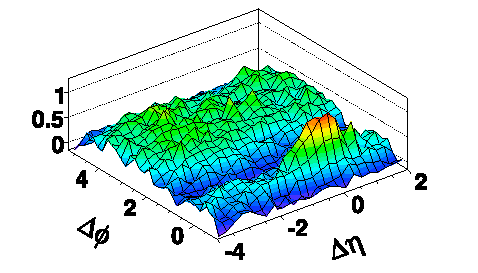
\includegraphics[width=.9\linewidth]{figs/PHOBOS-AuAu}
		\MyCite{Phys.Rev.Lett. 104, 062301}
		\\
		Многочастичные корреляции в AuAu столкновениях.
		\vskip.05\textheight
		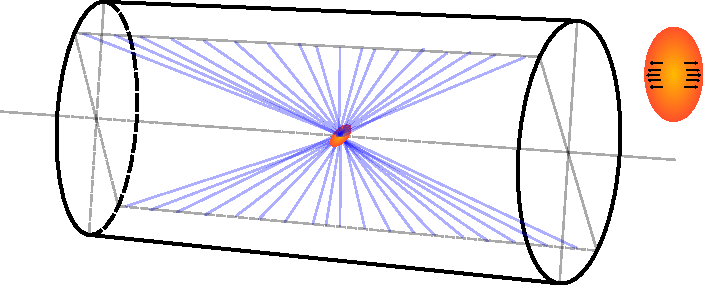
\includegraphics[width=\linewidth]{figs/ion-ridge}
	}
	\end{columns}
}

\frame{
	\frametitle{Кварк-глюонная плазма в $pp$ соударениях}
	\hfillstar \MyCiteHor{arXiv:1308.1435}\\
	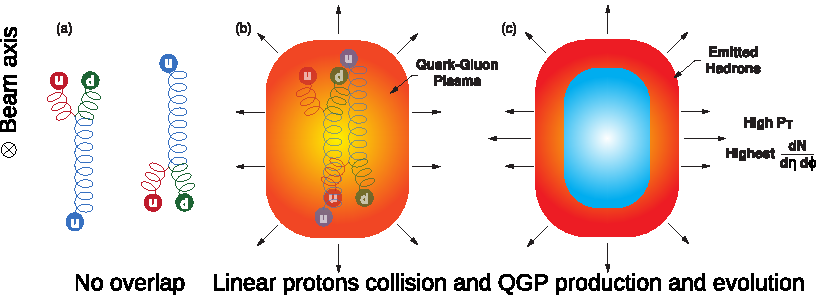
\includegraphics[width=\linewidth]{figs/pp-plasma}
	\vskip.5\baselineskip
	Можно предположить ненулевую вероятность, что протон представляет собой вытянутую глюонную струну, соединяющую кварк и дикварк. Если эта вероятность хотя бы 20\%, сечения хватит для объяснения зарегистрированных количеств частиц. 
}

\frame{
	\frametitle{Корреляции на самых ранних стадиях соударений}
	Ввиду большого расстояния между частицами, участвующими в дальних корреляциях, образование связи между ними должно происходить на самых ранних стадиях столкновения или даже до самого столкновения в волновых функциях сталкивающихся частиц. Первая из этих ситуаций может происходить в результате партонных рассеяний, поскольку существенный пик глюонных распределений происходит при рождении коллинеарных частиц. Причем распределение глюонов размывается при уменьшении $Q^2_s$, что объясняет отсутствие дальних корреляций частиц с малыми импульсами и при малых множественностях. 
	\\\hfillstar \MyCiteHor{arXiv:1201.2658}
}

\iffalse
\frame{
	\frametitle{Предельный переход в теории возмущений}
	\MyCite{arXiv:1105.3275}
	\hfillstar
	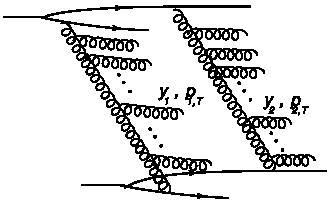
\includegraphics[width=.5\linewidth]{figs/pQCD-diagram}
	\hfillstar\\
	\hfillstar
	Диаграмма партонных ливней с $\Delta\phi\approx0$.
	\hfillstar
	\vskip.5\baselineskip
	Партонные ливни коррелированны, поскольку при вычислении сечения берется интеграл по поперечному обмениваемому импульсу $Q_T$. 
	Если предположить, что вероятность испускания глюона пропорциональна $\vec{Q}_T\cdot\vec{p}_T$, то естественным образом возникает коллимация ливней около $\Delta\phi=0$ и слагаемое $cos(2\Delta\phi$ в разложении 
}
\fi

\frame{
	\frametitle{Экспериментально изучаемые распределения}
	Назовем частицы в рассматриваемых парах $a$ и $b$.
	Помимо упомянутой величины $C(\Delta\eta,\Delta\phi) = \dfrac{S(\Delta\eta,\Delta\phi)}{B(\Delta\eta,\Delta\phi)}$ удобно рассматривать величину 
	$C(\Delta\phi) = \frac
		{\int\limits_2^5 S(\Delta\eta,\Delta\phi)\d\Delta\eta}
		{\int\limits_2^5 B(\Delta\eta,\Delta\phi)\d\Delta\eta}
	\equiv\dfrac{S(\Delta\phi)}{B(\Delta\phi)}$
	и кроме нее 
	$Y(\Delta\phi) = \frac
	{\int\limits_{-\pi/2}^{3\pi/2}B(\Delta\phi)\d\Delta\phi}
	{N_a\int\limits_{-\pi/2}^{3\pi/2}\d\Delta\phi}
	\,C(\Delta\phi),
	$
	где $N_a$ -- полное число частиц $a$. Тогда $Y(\Delta\phi)$ -- среднее число частиц $b$, соответствующих окрестности $\Delta\phi$.

	Для выявления вклада непосредственно хребта, $Y$ представляют в виде 
	$$
	Y(\Delta\phi) = Y^{\text{ridge}}(\Delta\phi) + Y^{\text{hard}}(\Delta\phi),
	$$$$
	Y^\text{ridge}(\Delta\phi) = G\left(1+\sum\limits_{n=2}^\infty2v_{n,n}\cos(n\Delta\phi)\right), 
	\quad
	Y^{\text{hard}}(\Delta\phi) = F\,\cos(\Delta\phi)
	$$
}

\frame{
	\frametitle{Попарная независимость частиц}
	Многочастичные корреляции могут появляться и при отсутствии связи между каждой парой частиц. Пусть одночастичное распределение
	$$\frac{\d N^\text{частиц}}{\d \phi} = \mathrm{const}\left(1+\sum\limits_{n}2v_n\cos\big(n(\phi-\psi_n)\big)\right),
	$$
	а двухчастичное
	$$
	\frac{\d N^\text{пар}}{\d \Delta\phi} = \mathrm{const}\left(1+\sum\limits_{n}2v_{n,n}\cos(n\Delta\phi)\right).
	$$
	Тогда, если двухчастичные корреляции отсутствуют, $v_{n,n} = v_n^2$ или $v_n(p_T^a)\,v_n(p_T^b)$
	
	\vskip.5\baselineskip
	В связи с этим также рассматривают ``одночастичные'' характеристики $$v_n(p_T^a) = v_{n,n}(p_T^a,p_T^b)\bigg/\sqrt{v_{n.n}(p_T^b,p_T^b)}$$
}

\frame{
	\frametitle{Хребты в $pp$ и $p\mathrm{Pb}$ соударениях}
	\centering
	\MyCite{arXiv:1609.06213}
	\hfillstar
	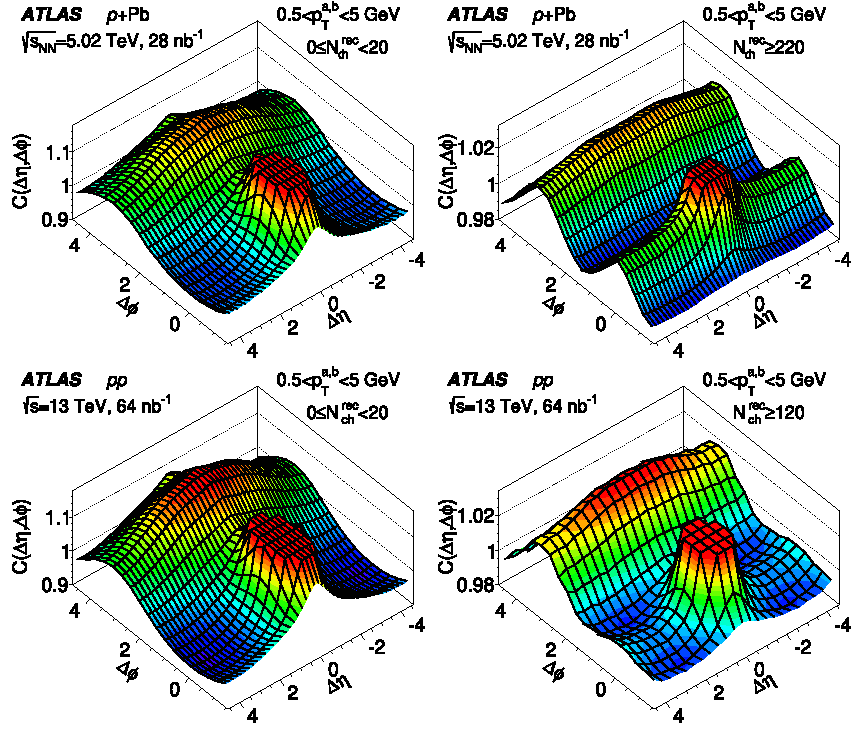
\includegraphics[height=.87\textheight]{figs/ATLAS-16}
	\hfillstar
}

\frame{
	\frametitle{Факторизация коэффициентов $v_{n,n}$}
	\def\tmpVariable{
		\MyCite{arXiv:1609.06213}
		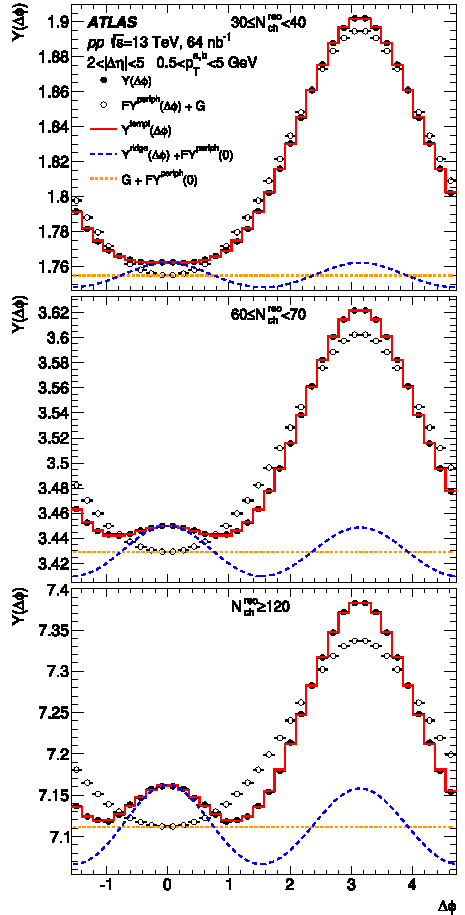
\includegraphics[height=.87\textheight]{figs/ATLAS-Y-pp}
	}
	\begin{columns}
	\column{\widthof{\tmpVariable}}{
		\tmpVariable
	}
	\column{\linewidth-\widthof{\tmpVariable}}{
		\centering
		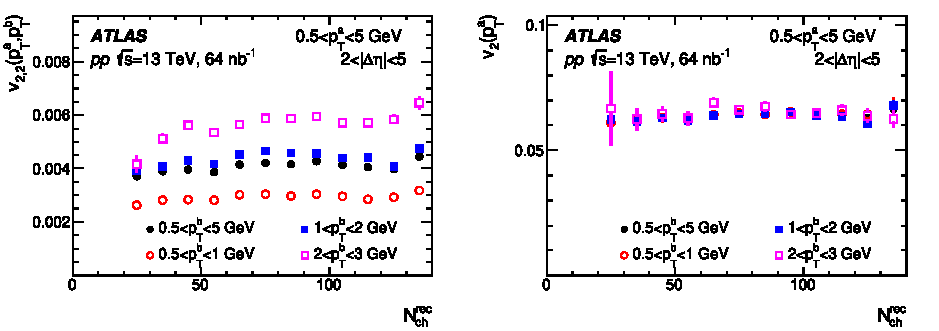
\includegraphics[width=\linewidth]{figs/ATLAS-vnnvn-pp}\\
		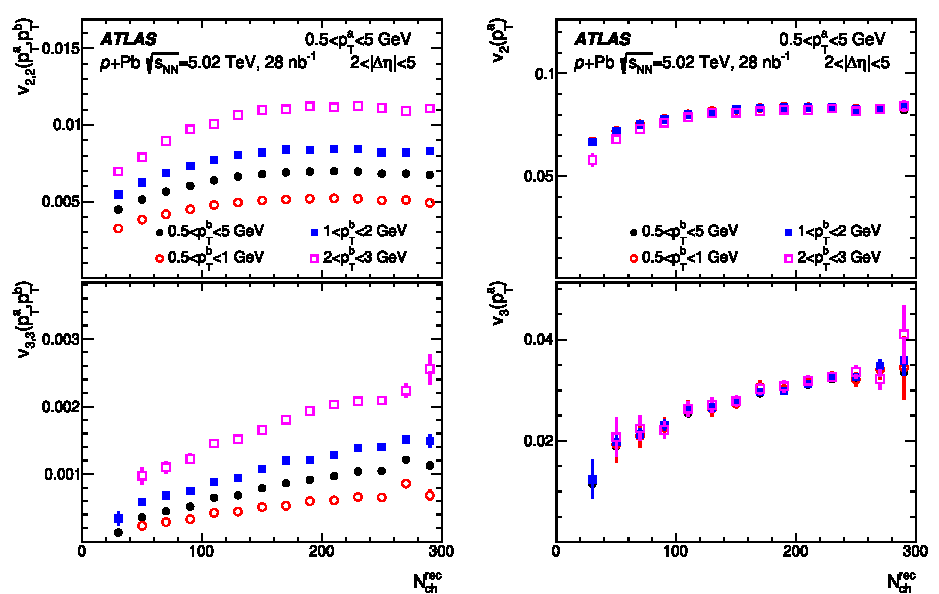
\includegraphics[width=\linewidth]{figs/ATLAS-vnnvn-pPb}\\
	}
	\end{columns}
}

\frame{
	\frametitle{Различия $pp$ и $p\mathrm{Pb}$ соударений}
	\begin{columns}
	\column[t]{.6\linewidth}{
		Форма распределения частиц в $pp$ соударениях не зависит от множественности в событии, то есть большая множественность в событиях обусловлена явлениями, имеющими то же азимутальное распределение, что и уже известные. В $p\mathrm{Pb}$ соударениях оно меняется -- становится более вытянутым. 
	}
	\column[t]{.4\linewidth}{
		\vskip-\baselineskip
		\hfillstar
		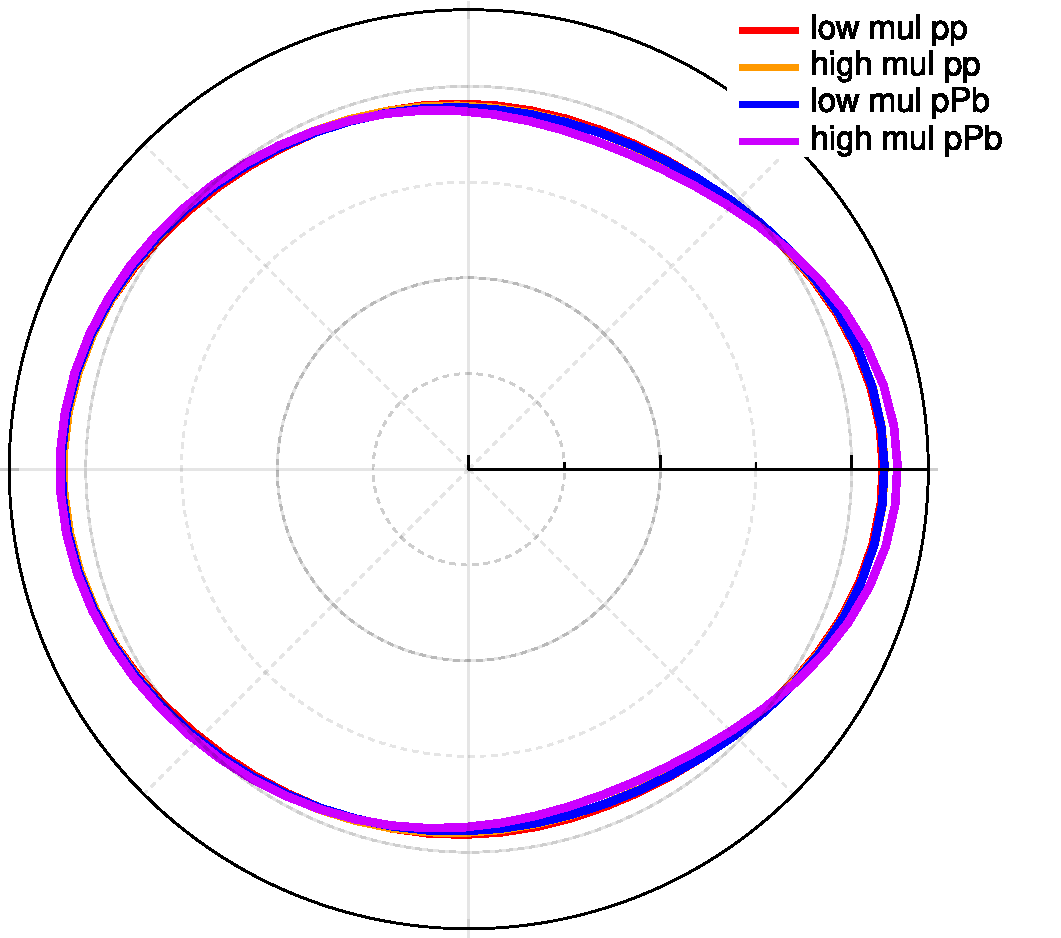
\includegraphics[width=\linewidth]{figs/Y-polar}
	}
	\end{columns}
	\vskip-.5\baselineskip
	\hfillstar\MyCiteHor{arXiv:1609.06213}
	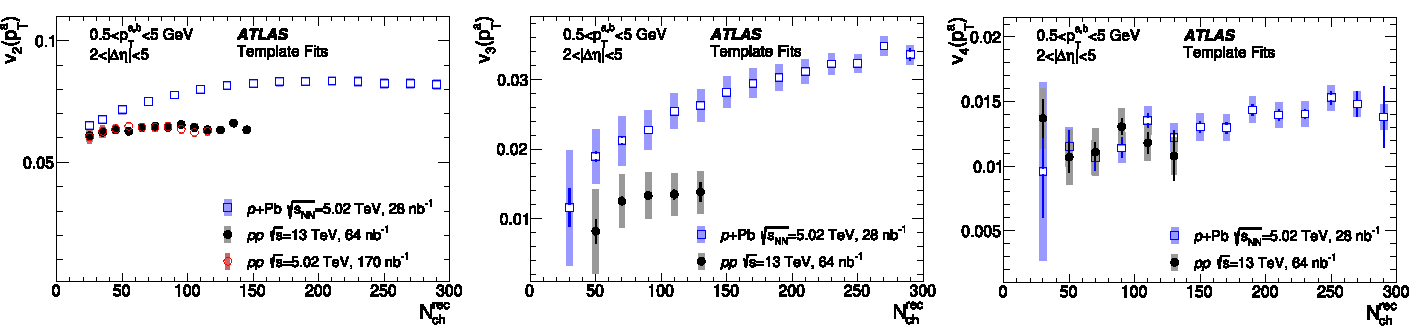
\includegraphics[width=\linewidth]{figs/ATLAS-vn}
}

\frame{
	\frametitle{Выводы}
	\begin{itemize}
	\item Приведена принципиальная форма функции, отражающей многочастичные корреляции.
	\item Успешно описаны процессы, дающие вклад в корреляцию в $pp$ соударениях с малой множественностью.
	\item Рассмотрены изменения корреляций при увеличении множественности и поперечных импульсов частиц в событиях.
	\item Описаны пик при $\Delta\phi=0$, $\Delta\eta=0$ и широкий хребет при $\Delta\phi=\pi$.
	\item Рассмотрены и удовлетворительно объяснены односторонние дальние корреляции (хребет при $\Delta\phi=0$) в ядро-ядерных соударениях.
	\item Показаны способы описания аналогичных корреляций в протонных соударениях. 
	\item Проведено сравнение протонных и протон-ядерных соударений при различных множественностях. Распределения частиц не идентичны. 
	\end{itemize}
}

\end{document}



	\begin{columns}
	\column{.5\linewidth}{

	}
	\column{.5\linewidth}{

	}
	\end{columns}


% this slide is not for this topic of presentation
\iffalse
\frame{
	\frametitle{Что показывают на графиках}
	% Упомянуть, что быстротой названа псевдобыстрота
	Плотность распределения числа частиц по быстроте для одной частицы приблизительно константа и не зависит от быстроты. Плотность вероятности разности быстрот двух независимых частиц, полученная на основании уже упомянутой плотности интегрированием, имеет пик несмотря на независимость частиц. Для выявления корреляций в распределении зависимых частиц необходимо учесть форму распределения независимых. 
	$$
	\frac{\d n^{\text{частиц}}}{\d \eta} \approx \left\{ 
	\begin{array}{ll}
		\mathrm{const}, & \eta \in (-2.5, 2.5) \\
		0, & \eta \notin (-2.5, 2.5)
	\end{array}\right.
	\: \Rightarrow \:
	\frac{\d n^{\text{пар, незав}}}{\d (\eta_1 - \eta_2)} \approx \text{треугольник}
	$$

	Аналогичные соображения применимы и к азимутальному углу. В итоге
	$$
	C(\Delta\eta, \Delta\phi) = \frac{n^2}{n(n-1)}\,{\d n^{\text{зав}} \over \d n^{\text{незав}}} 
	\;\text{или}\;
	\frac{1}{n(n-1)}{\d n^{\text{зав}} \over \d\Delta\eta\,\d\Delta\phi} -	\frac{1}{n^2}{\d n^{\text{незав}} \over \d\Delta\eta\,\d\Delta\phi}
	$$
	будет отражать двухчастичные корреляции. 
}
\fi

